\documentclass[aspectratio=169,11pt,t]{beamer}

% ============================================================
% Theme and typography
% ============================================================

\usetheme{Madrid}
\usecolortheme{default}
\usefonttheme{professionalfonts}

\setbeamertemplate{navigation symbols}{}
\setbeamertemplate{headline}{}

\setbeamertemplate{footline}{%
  \leavevmode\hbox{%
  \begin{beamercolorbox}[wd=.82\paperwidth,ht=2.5ex,dp=1.0ex,leftskip=.8em]{author in head/foot}
    CSCI 6461 --- Computer Systems Architecture (AArch64 Reference / RISC Philosophy)
  \end{beamercolorbox}%
  \begin{beamercolorbox}[wd=.18\paperwidth,ht=2.5ex,dp=1.0ex,rightskip=.8em]{date in head/foot}
    \hfill\insertframenumber/\inserttotalframenumber
  \end{beamercolorbox}}
}

\setbeamersize{
  text margin left=0.65cm,
  text margin right=0.65cm
}

\setbeamerfont{frametitle}{size=\Large, series=\bfseries}
\setbeamerfont{block title}{size=\normalsize, series=\bfseries}
\setbeamertemplate{blocks}[rounded][shadow=false]

% Block vertical padding adjustments
\addtobeamertemplate{block begin}{\vspace{0pt}}{\vspace{0pt}}
\addtobeamertemplate{block end}{}{\vspace{0.15em}}

% Base list item separation
\setbeamertemplate{itemize/enumerate body begin}{\setlength{\itemsep}{3pt}}
\setbeamertemplate{itemize/enumerate subbody begin}{\setlength{\itemsep}{1.5pt}}

% ============================================================
% Packages
% ============================================================

\usepackage[T1]{fontenc}
\usepackage{lmodern}
\usepackage{amsmath}
\usepackage{booktabs}
\usepackage{array}
\usepackage{tikz}

\usetikzlibrary{
  arrows.meta,
  positioning,
  shapes.geometric,
  calc,
  decorations.pathreplacing
}

% ============================================================
% Colors
% ============================================================

\definecolor{navy}{RGB}{24,43,68}
\definecolor{deepblue}{RGB}{45,88,130}
\definecolor{lightblue}{RGB}{235,242,250}
\definecolor{softgray}{RGB}{245,247,250}
\definecolor{darkgray}{RGB}{25,28,32}
\definecolor{gold}{RGB}{200,145,35}

\setbeamercolor{palette primary}{bg=navy,fg=white}
\setbeamercolor{palette secondary}{bg=deepblue,fg=white}
\setbeamercolor{frametitle}{bg=navy,fg=white}
\setbeamercolor{title}{fg=white}
\setbeamercolor{subtitle}{fg=white}
\setbeamercolor{author}{fg=white}
\setbeamercolor{date}{fg=white}
\setbeamercolor{titlelike}{fg=white}
\setbeamercolor{block title}{bg=deepblue,fg=white}
\setbeamercolor{block body}{bg=lightblue,fg=darkgray}
\setbeamercolor{normal text}{fg=darkgray,bg=white}

% ============================================================
% Formatting shortcuts
% ============================================================

\setlength{\parskip}{0pt}

\newcommand{\key}[1]{\textbf{#1}}
\newcommand{\bits}[1]{\texttt{#1}}
\newcommand{\hex}[1]{\texttt{0x#1}}
\newcommand{\code}[1]{\texttt{#1}}

% Section divider macro
\newcommand{\sectiondivider}[2]{%
\begin{frame}[plain]
\begin{tikzpicture}[remember picture,overlay]
\fill[navy] (current page.south west) rectangle (current page.north east);
\fill[gold] (current page.south west) rectangle ([yshift=.15cm]current page.south east);
\end{tikzpicture}
\vspace*{\fill}
\begin{minipage}{0.85\textwidth}
{\color{gold}\large\bfseries #1\par}
\vspace{0.3cm}
{\color{white}\fontsize{22}{26}\selectfont\bfseries #2\par}
\end{minipage}
\vspace*{\fill}
\end{frame}
}

% ============================================================
% Metadata
% ============================================================

\title[Topic 3]{
  The Hardware/Software Interface\\
  \& AArch64 Programmer's Model
}

\subtitle{
  Architectural state, registers, memory organization,
  and foundational instruction mechanics
}

\author{
  Computer Systems Architecture
}

\date{}

% ============================================================
% Document
% ============================================================

\begin{document}

% ============================================================
% Slide 1: Title Slide
% ============================================================

\begin{frame}[plain]
\begin{tikzpicture}[remember picture,overlay]
\fill[navy] (current page.south west) rectangle (current page.north east);
\fill[gold] (current page.south west) rectangle ([yshift=.15cm]current page.south east);
\end{tikzpicture}

\vspace*{\fill}
\begin{minipage}{0.88\textwidth}
{\color{gold}\normalsize\bfseries CSCI 6461 \;|\; TOPIC 3\par}
\vspace{0.25cm}
{\color{white}\fontsize{24}{28}\selectfont\bfseries
 The Hardware/Software Interface\\[0.08cm]
 \& AArch64 Programmer's Model
\par}
\vspace{0.35cm}
{\color{white!80}\large
 Architectural state, registers, memory organization,
 and foundational instruction mechanics
\par}
\end{minipage}

\vfill
{\color{white}\normalsize Dr. J. Burns\par}
{\color{white!70}\small Computer Systems Architecture --- AArch64 Reference Platform\par}
\vspace*{\fill}
\end{frame}

% ============================================================
% Slide 2: Module Topics
% ============================================================

\begin{frame}{Topic 3: Module Topics}
\vfill
\begin{enumerate}\setlength{\itemsep}{7pt}
  \item \key{Architectural State \& The Hardware Contract}
  \begin{itemize}
    \item Concrete definition of architectural state vs.\ microarchitectural structures.
    \item The AArch64 programmer's model and processor execution modes.
  \end{itemize}

  \item \key{AArch64 Register File \& Naming Conventions}
  \begin{itemize}
    \item The 31 general-purpose registers: 64-bit (\bits{x0}--\bits{x30}) vs.\ 32-bit (\bits{w0}--\bits{w30}).
    \item Special-purpose registers: Zero register (\bits{xzr}/\bits{wzr}), stack pointer (\bits{sp}), program counter (\bits{pc}).
    \item Standard ABI register usage: arguments, return values, caller-saved, and callee-saved registers.
  \end{itemize}

  \item \key{Memory Organization \& Endianness}
  \begin{itemize}
    \item Byte-addressable 64-bit address space, memory alignment rules, and byte ordering.
  \end{itemize}

  \item \key{Core Instruction Classes \& Execution Mechanics}
  \begin{itemize}
    \item Data movement, arithmetic/logical operations, NZCV condition flags, and condition codes.
  \end{itemize}
\end{enumerate}
\vfill
\end{frame}

% ============================================================
% Section 1 Divider
% ============================================================

\sectiondivider{PART 1}{Architectural State \& Execution Model}

% ============================================================
% Slide 3
% ============================================================

\begin{frame}{What Is Architectural State?}
\vfill
\begin{itemize}\setlength{\itemsep}{4pt}
  \item \key{Definition:} The complete set of software-visible hardware storage locations required to represent a program's execution at any discrete point in time.
  \item If execution is interrupted (context switch, interrupt, exception), saving and restoring this exact state allows program resumption without alteration of behavior.
  \item \key{Core Components in AArch64:}
  \begin{itemize}\setlength{\itemsep}{2pt}
    \item General-Purpose Registers (\bits{x0}--\bits{x30}).
    \item Program Counter (\bits{pc}) and Stack Pointer (\bits{sp}).
    \item Current Program Status Register / Condition Flags (\bits{pstate} / NZCV).
    \item System control and configuration registers (e.g., $\text{TTBR0\_EL1}$, $\text{SCTLR\_EL1}$ for memory management).
    \item Byte-addressed memory contents.
  \end{itemize}
\end{itemize}

\vfill
\begin{block}{State Checkpointing}
\small Operating systems actively rely on the strict definition of architectural state to successfully suspend and resume millions of threads per second without computational corruption.
\end{block}
\vfill
\end{frame}

% ============================================================
% Slide 4
% ============================================================

\begin{frame}{Architectural vs.\ Microarchitectural State}
\vfill
\begin{columns}[T]
\begin{column}{0.48\textwidth}
\begin{block}{Architectural State (Visible Contract)}
\small
\begin{itemize}\setlength{\itemsep}{3pt}
  \item Defined strictly by the ISA specification.
  \item Software directly reads/writes this state.
  \item \key{Examples:} Registers \bits{x0}--\bits{x30}, \bits{pc}, architectural memory, NZCV flags.
\end{itemize}
\end{block}
\end{column}

\begin{column}{0.48\textwidth}
\begin{block}{Microarchitectural State (Hidden)}
\small
\begin{itemize}\setlength{\itemsep}{3pt}
  \item Internal hardware implementation details.
  \item Invisible to software correctness.
  \item \key{Examples:} Pipeline latches, L1/L2 caches, Branch Target Buffers, rename tables.
\end{itemize}
\end{block}
\end{column}
\end{columns}

\vfill
\begin{block}{The Execution Boundary}
\small Hardware may execute instructions out of order across hidden microarchitectural buffers, but it \key{must} commit all final results sequentially to the visible architectural state.
\end{block}
\vfill
\end{frame}

% ============================================================
% Slide 5
% ============================================================

\begin{frame}{The AArch64 Execution State}
\vfill
\begin{itemize}\setlength{\itemsep}{6pt}
  \item \key{AArch64:} Pure 64-bit execution state introduced in ARMv8-A.
  \item \key{Flat 64-bit Virtual Addressing:} Registers hold 64-bit pointers (architectural address space up to $2^{64}$ bytes). Fixed 4-byte instruction width remains permanently aligned to 4-byte memory boundaries.
  \item \key{Clean-Slate RISC Design:} Eliminates legacy A32 quirks by removing universal conditional execution, removing \code{ldm}/\code{stm} loops, and decoupling the Program Counter (\bits{pc}) entirely from the general register file.
\end{itemize}

\vfill
\begin{block}{The Legacy-Free Advantage}
\small By abandoning strict backwards compatibility with 32-bit ARM inside the AArch64 execution mode, engineers freed up massive decode logic and instruction-encoding space.
\end{block}
\vfill
\end{frame}

% ============================================================
% Slide 6 (Expanded Full-Height Hierarchy & Privilege Model)
% ============================================================

\begin{frame}{Privilege Levels (Exception Levels)}
\vfill
\begin{columns}[T,onlytextwidth]
\begin{column}{0.46\textwidth}
\centering
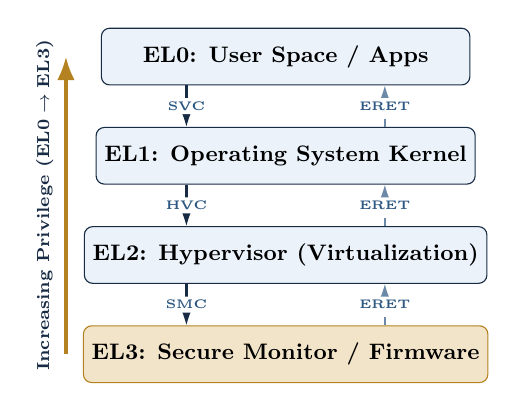
\begin{tikzpicture}[
  scale=0.90,
  every node/.style={transform shape},
  elbox/.style={
    draw=navy,
    fill=lightblue,
    rounded corners=3pt,
    font=\small\bfseries,
    minimum width=5.2cm,
    minimum height=0.80cm,
    align=center
  },
  el3box/.style={
    draw=gold!90!black,
    fill=gold!25,
    rounded corners=3pt,
    font=\small\bfseries,
    minimum width=5.2cm,
    minimum height=0.80cm,
    align=center
  },
  translabel/.style={
    font=\tiny\bfseries,
    text=deepblue,
    fill=white,
    inner sep=1.5pt,
    rounded corners=1pt
  }
]
  % Exception Level Nodes (Full vertical spacing)
  \node[elbox] (el0) at (0, 4.2) {EL0: User Space / Apps};
  \node[elbox] (el1) at (0, 2.8) {EL1: Operating System Kernel};
  \node[elbox] (el2) at (0, 1.4) {EL2: Hypervisor (Virtualization)};
  \node[el3box] (el3) at (0, 0.0) {EL3: Secure Monitor / Firmware};

  % Escalation Paths (Traps, Syscalls, Exceptions)
  \draw[-{Latex[length=2.5mm]}, thick, navy] ([xshift=-1.4cm]el0.south) -- ([xshift=-1.4cm]el1.north)
    node[midway, translabel] {SVC};
  \draw[-{Latex[length=2.5mm]}, thick, navy] ([xshift=-1.4cm]el1.south) -- ([xshift=-1.4cm]el2.north)
    node[midway, translabel] {HVC};
  \draw[-{Latex[length=2.5mm]}, thick, navy] ([xshift=-1.4cm]el2.south) -- ([xshift=-1.4cm]el3.north)
    node[midway, translabel] {SMC};

  % De-escalation Return Paths (ERET)
  \draw[-{Latex[length=2.5mm]}, thick, deepblue!70, dashed] ([xshift=1.4cm]el1.north) -- ([xshift=1.4cm]el0.south)
    node[midway, translabel] {ERET};
  \draw[-{Latex[length=2.5mm]}, thick, deepblue!70, dashed] ([xshift=1.4cm]el2.north) -- ([xshift=1.4cm]el1.south)
    node[midway, translabel] {ERET};
  \draw[-{Latex[length=2.5mm]}, thick, deepblue!70, dashed] ([xshift=1.4cm]el3.north) -- ([xshift=1.4cm]el2.south)
    node[midway, translabel] {ERET};

  % Privilege Level Axis
  \draw[-{Latex[length=3mm]}, line width=1.2pt, gold!90!black] (-3.1, 0.0) -- (-3.1, 4.2);
  \node[rotate=90, font=\scriptsize\bfseries, text=navy] at (-3.4, 2.1) {Increasing Privilege ($\text{EL0} \to \text{EL3}$)};
\end{tikzpicture}
\begin{block}{CSCI 6461 Scope}
\small Analysis focuses on \key{EL0} execution mechanics and the \key{EL0 $\to$ EL1} system call boundary.
\end{block}
\end{column}

\begin{column}{0.52\textwidth}
\small
\begin{itemize}\setlength{\itemsep}{5pt}
  \item \key{EL0 (Application):} Unprivileged user space executing application logic with private virtual address spaces.
  \item \key{EL1 (OS Kernel):} Privileged kernel execution managing memory translation, drivers, and process scheduling
  \item \key{EL2 (Hypervisor):} Non-secure virtualization layer enforcing second-stage address translation across guest OS instances
  \item \key{EL3 (Secure Monitor):} Root security layer hosting firmware and managing ARM TrustZone secure-world switching
\end{itemize}

\end{column}
\end{columns}
\vfill
\end{frame}

% ============================================================
% Section 2 Divider
% ============================================================

\sectiondivider{PART 2}{AArch64 Register Architecture \& ABI}

% ============================================================
% Slide 7
% ============================================================

\begin{frame}{General-Purpose Registers: \texttt{x0}--\texttt{x30}}
\vfill
\begin{itemize}\setlength{\itemsep}{4pt}
  \item AArch64 provides \key{31 general-purpose registers} (\bits{x0}--\bits{x30}), each exactly \key{64 bits wide} ($8\text{ bytes}$).
  \item \key{Orthogonal Design:} Any of these registers can serve interchangeably as a source, destination, or base address pointer without restriction.
  \item \key{Simplified ISA:} Eliminates dedicated register constraints (e.g., implicit counter registers) found in legacy architectures like x86.
\end{itemize}

\vfill
\centering
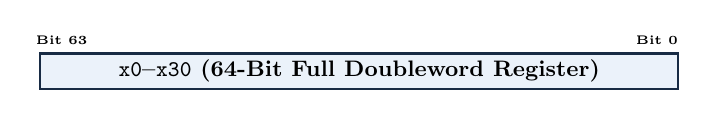
\begin{tikzpicture}[scale=0.9, every node/.style={transform shape}]
  \draw[fill=lightblue, draw=navy, thick] (0,0) rectangle (9.0,0.5);
  \node at (4.5, 0.25) {\small\textbf{\texttt{x0}--\texttt{x30} (64-Bit Full Doubleword Register)}};
  \node[anchor=south, font=\tiny\bfseries] at (0.3, 0.5) {Bit 63};
  \node[anchor=south, font=\tiny\bfseries] at (8.7, 0.5) {Bit 0};
\end{tikzpicture}

\vfill
\begin{block}{Why Exactly 31 Registers?}
\small RISC instructions allocate 5 bits for register operands ($2^5 = 32$). AArch64 dedicates 31 slots to general storage and reserves the 32nd slot for a Zero Register / Stack Pointer alias.
\end{block}
\vfill
\end{frame}

% ============================================================
% Slide 8
% ============================================================

\begin{frame}{32-Bit Register Views: \texttt{w0}--\texttt{w30}}
\vfill
\begin{itemize}\setlength{\itemsep}{4pt}
  \item Every 64-bit \bits{x} register has a corresponding 32-bit view denoted as \bits{w0} through \bits{w30}.
  \item \bits{wN} represents the \key{lower 32 bits (bits 31:0)} of the physical register \bits{xN}.
  \item Enables native 32-bit integer arithmetic without requiring separate hardware register files.
\end{itemize}

\vfill
\centering
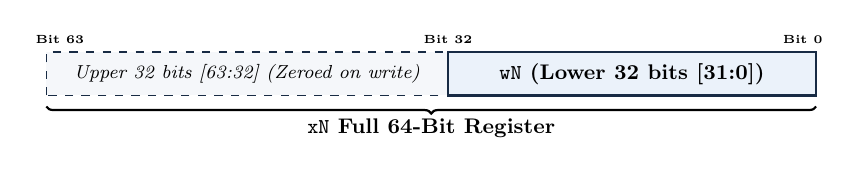
\begin{tikzpicture}[scale=0.85, every node/.style={transform shape}]
  \draw[fill=softgray, draw=navy, dashed] (0,0) rectangle (6.0,0.65);
  \node at (3.0, 0.325) {\footnotesize\textit{Upper 32 bits [63:32] (Zeroed on write)}};
  \draw[fill=lightblue, draw=navy, thick] (6.0,0) rectangle (11.5,0.65);
  \node at (8.75, 0.325) {\small\textbf{\texttt{wN} (Lower 32 bits [31:0])}};
  \node[anchor=south, font=\tiny\bfseries] at (0.2, 0.65) {Bit 63};
  \node[anchor=south, font=\tiny\bfseries] at (6.0, 0.65) {Bit 32};
  \node[anchor=south, font=\tiny\bfseries] at (11.3, 0.65) {Bit 0};
  \draw[thick, decoration={brace, mirror, raise=4pt}, decorate] (0,0) -- (11.5,0) node[midway, below=6pt, font=\small\bfseries] {\texttt{xN} Full 64-Bit Register};
\end{tikzpicture}

\vfill
\begin{block}{Zero-Extension Safety Rule}
\small Writing any data to a 32-bit \bits{w} register \key{automatically zero-extends} the value, completely clearing the upper 32 bits of the corresponding \bits{x} register to eliminate stale garbage data.
\end{block}
\vfill
\end{frame}

% ============================================================
% Slide 9
% ============================================================

\begin{frame}{The Zero Register: \texttt{xzr} and \texttt{wzr}}
\vfill
\begin{itemize}\setlength{\itemsep}{4pt}
  \item Encoded as register number 31 within standard ALU instruction encodings.
  \item \key{Read Behavior:} Always returns constant zero (\bits{0} for \bits{xzr}, 32-bit \bits{0} for \bits{wzr}).
  \item \key{Write Behavior:} Silently discards values written to it (serves as a discard bit-bucket).
  \item \key{Architectural Benefit:} Eliminates dedicated zero-loading and comparison instruction formats.
\end{itemize}

\vfill
\begin{block}{Common Idioms Using the Zero Register}
\small
\begin{tabular}{lll}
\toprule
\textbf{Assembly Instruction} & \textbf{Equivalent Operation} & \textbf{Purpose} \\
\midrule
\code{mov x0, xzr}            & $x_0 \leftarrow 0$            & Clear register $x_0$ to zero \\
\code{subs xzr, x1, x2}       & Evaluate $x_1 - x_2 \to \text{flags}$ & Compare $x_1$ and $x_2$ (alias: \code{cmp x1, x2}) \\
\code{str xzr, [x1]}          & $\text{Mem}[x_1] \leftarrow 0$ & Zero out a 64-bit memory word \\
\bottomrule
\end{tabular}
\end{block}
\vfill
\end{frame}

% ============================================================
% Slide 10
% ============================================================

\begin{frame}{Special-Purpose Registers: \texttt{sp}, \texttt{pc}, \texttt{lr}}
\vfill
\begin{columns}[T]
\begin{column}{0.48\textwidth}
\begin{block}{Stack Pointer (\texttt{sp})}
\small
\begin{itemize}\setlength{\itemsep}{3pt}
  \item Dedicated register holding stack top address.
  \item Must maintain \key{16-byte alignment} in the ABI.
  \item Restricted to stack allocation/deallocation.
\end{itemize}
\end{block}
\end{column}

\begin{column}{0.48\textwidth}
\begin{block}{Program Counter (\texttt{pc})}
\small
\begin{itemize}\setlength{\itemsep}{3pt}
  \item Holds address of current instruction.
  \item \key{Cannot} be read/written as data (\code{no mov x0, pc}).
  \item Accessed via PC-relative addressing (\code{adrp}).
  \item Modified via branch/call instructions.
\end{itemize}
\end{block}
\end{column}
\end{columns}

\vfill
\begin{block}{Link Register (\texttt{x30} / \texttt{lr})}
\small Holds the subroutine return address generated by branch-with-link (\code{bl}, \code{blr}). A function returns execution by branching to this register (\code{ret}).
\end{block}
\vfill
\end{frame}

% ============================================================
% Slide 11
% ============================================================

\begin{frame}{The Calling Convention: Caller- vs.\ Callee-Saved}
\vfill
\begin{columns}[T]
\begin{column}{0.48\textwidth}
\begin{block}{Caller-Saved Registers (\texttt{x0}--\texttt{x17})}
\small
\begin{itemize}\setlength{\itemsep}{3pt}
  \item Used for arguments and temporary scratch math.
  \item Caller \key{must save them} to stack before calls if values are needed later.
  \item Callee may overwrite them freely.
\end{itemize}
\end{block}
\end{column}

\begin{column}{0.48\textwidth}
\begin{block}{Callee-Saved Registers (\texttt{x19}--\texttt{x28})}
\small
\begin{itemize}\setlength{\itemsep}{3pt}
  \item Preserves long-lived variables across calls.
  \item If callee modifies these, it \key{must save and restore} their original contents.
  \item Guarantees protection of caller state.
\end{itemize}
\end{block}
\end{column}
\end{columns}

\vfill
\begin{block}{The Efficiency Trade-off}
\small Balancing caller- and callee-saved registers across the ABI minimizes memory traffic and stack spilling during nested subroutine calls.
\end{block}
\vfill
\end{frame}

% ============================================================
% Slide 12
% ============================================================

\begin{frame}{AArch64 Register File Overview}
\vfill
\begin{center}
\scriptsize
\renewcommand{\arraystretch}{0.92}
\setlength{\tabcolsep}{4pt}
\begin{tabular}{lll}
\toprule
\textbf{Register} & \textbf{Architectural Role} & \textbf{Preserved Across Calls? (ABI)} \\
\midrule
\bits{x0}--\bits{x7}   & Function arguments \& return values                     & No (Caller-saved / Scratch) \\
\bits{x8}              & Indirect result location (struct return pointer)        & No (Caller-saved) \\
\bits{x9}--\bits{x15}  & Temporary / Scratch registers                           & No (Caller-saved) \\
\bits{x16}--\bits{x17} & Intra-procedure-call temporary registers (IP0, IP1)     & No (Caller-saved) \\
\bits{x18}             & Platform register (reserved for OS / TLS)               & Platform-dependent \\
\bits{x19}--\bits{x28} & Callee-saved registers                                  & \key{Yes (Callee-saved)} \\
\bits{x29} (\bits{fp}) & Frame pointer (base of current stack frame)             & \key{Yes (Callee-saved)} \\
\bits{x30} (\bits{lr}) & Link register (subroutine return address)               & No (Caller-saved) \\
\bits{sp}              & Dedicated stack pointer (16-byte aligned)              & \key{Yes (Preserved)} \\
\bits{xzr}             & Dedicated zero register (constant 0, writes discarded) & N/A (Hardware constant) \\
\bottomrule
\end{tabular}
\end{center}
\vfill
\end{frame}

% ============================================================
% Slide 13
% ============================================================

\begin{frame}{Process State: \texttt{pstate} and Condition Flags}
\vfill
\begin{itemize}\setlength{\itemsep}{3pt}
  \item The processor maintains an internal process state register (\bits{pstate}).
  \item The upper 4 bits evaluate the \key{NZCV Arithmetic Condition Flags}:
\end{itemize}

\vfill
\begin{center}
\footnotesize
\setlength{\tabcolsep}{6pt}
\begin{tabular}{cll}
\toprule
\textbf{Flag} & \textbf{Name} & \textbf{Condition Under Which Flag Is Set to 1} \\
\midrule
\key{N} & \textbf{Negative} & Result bit 63 (or bit 31) is 1 (negative signed value) \\
\key{Z} & \textbf{Zero}     & Computed result is exactly zero \\
\key{C} & \textbf{Carry}    & Operation generated an unsigned carry-out (or no borrow in sub) \\
\key{V} & \textbf{Overflow} & Signed arithmetic overflow occurred (sign bit is invalid) \\
\bottomrule
\end{tabular}
\end{center}

\vfill
\begin{block}{Selective Flag Updates}
\small Standard ALU instructions (\code{add}, \code{sub}) do \key{not} modify flags. Only instructions with an ``\code{s}'' suffix (\code{adds}, \code{subs}) or comparison instructions (\code{cmp}) update NZCV.
\end{block}
\vfill
\end{frame}

% ============================================================
% Section 3 Divider
% ============================================================

\sectiondivider{PART 3}{Memory Model, Alignment \& Endianness}

% ============================================================
% Slide 14
% ============================================================

\begin{frame}{Memory Organization \& Byte Addressing}
\vfill
\begin{itemize}\setlength{\itemsep}{3pt}
  \item Memory is organized physically as a contiguous sequence of \key{8-bit bytes}.
  \item Every individual byte is assigned a unique 64-bit architectural address.
  \item Data operands span consecutive byte addresses scaling by standard powers of two:
\end{itemize}

\vfill
\begin{center}
\footnotesize
\renewcommand{\arraystretch}{1.0}
\setlength{\tabcolsep}{8pt}
\begin{tabular}{lcll}
\toprule
\textbf{Data Type} & \textbf{Size (Bytes)} & \textbf{Size (Bits)} & \textbf{AArch64 Architecture Term} \\
\midrule
Byte         & 1  & 8-bit  & Byte (\code{b}) \\
Halfword     & 2  & 16-bit & Halfword (\code{h}) \\
Word         & 4  & 32-bit & Word (\code{w}) \\
Doubleword   & 8  & 64-bit & Doubleword (\code{x}) \\
Quadword     & 16 & 128-bit& Quadword / Vector element (\code{q}) \\
\bottomrule
\end{tabular}
\end{center}

\vfill
\begin{block}{64-Bit Pointer Translation}
\small While pointers are architecturally 64 bits wide, current hardware implementations cap physical virtual addressing to 48 or 52 bits to reduce page-table traversal costs.
\end{block}
\vfill
\end{frame}

% ============================================================
% Slide 15
% ============================================================

\begin{frame}{Memory Alignment Rules}
\vfill
\begin{itemize}\setlength{\itemsep}{3pt}
  \item An access to an $n$-byte operand is \key{naturally aligned} if $\text{Address} \pmod n = 0$.
  \item \textbf{Alignment Rules:} Word ($4\text{B}$ boundary), Doubleword ($8\text{B}$ boundary), Instruction fetch ($4\text{B}$ boundary).
\end{itemize}

\vfill
\begin{columns}[T]
\begin{column}{0.48\textwidth}
\begin{block}{Aligned Access (Single Transaction)}
\centering
\vspace{0.05cm}
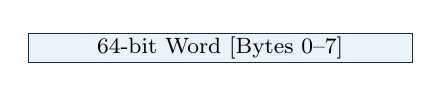
\begin{tikzpicture}[scale=0.75]
  \draw[fill=lightblue, draw=navy] (0,0) rectangle (6.5,0.5) node[midway, font=\footnotesize] {64-bit Word [Bytes 0--7]};
\end{tikzpicture}
\end{block}
\end{column}

\begin{column}{0.48\textwidth}
\begin{block}{Unaligned Access (Crosses Boundary)}
\centering
\vspace{0.05cm}
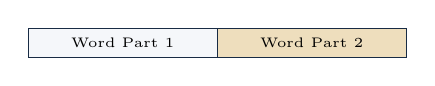
\begin{tikzpicture}[scale=0.75]
  \draw[fill=softgray, draw=navy] (0,0) rectangle (3.2,0.5) node[midway, font=\tiny] {Word Part 1};
  \draw[fill=gold!30, draw=navy] (3.2,0) rectangle (6.4,0.5) node[midway, font=\tiny] {Word Part 2};
\end{tikzpicture}
\end{block}
\end{column}
\end{columns}

\vfill
\begin{block}{Alignment Penalties}
\small Unaligned memory accesses can cross cache-line boundaries, requiring multiple memory transactions and degrading bandwidth. Strict environments raise a hardware fault on unaligned access.
\end{block}
\vfill
\end{frame}

% ============================================================
% Slide 16
% ============================================================

\begin{frame}{Byte Ordering: Little-Endian vs.\ Big-Endian}
\vfill
\small Storage of 32-bit Word \hex{0a0b0c0d} at Base Address \hex{1000}:

\vfill
\begin{columns}[T]
\begin{column}{0.48\textwidth}
\begin{block}{Little-Endian (AArch64 Default)}
\begin{itemize}\setlength{\itemsep}{2pt}
  \item \key{Least Significant Byte (LSB)} stored at the \key{lowest} memory address.
\end{itemize}
\centering
\footnotesize
\begin{tabular}{cc}
\toprule
\textbf{Address} & \textbf{Stored Byte} \\
\midrule
\hex{1000} & \hex{0d} (LSB) \\
\hex{1001} & \hex{0c} \\
\hex{1002} & \hex{0b} \\
\hex{1003} & \hex{0a} (MSB) \\
\bottomrule
\end{tabular}
\end{block}
\end{column}

\begin{column}{0.48\textwidth}
\begin{block}{Big-Endian (Network Order)}
\begin{itemize}\setlength{\itemsep}{2pt}
  \item \key{Most Significant Byte (MSB)} stored at the \key{lowest} memory address.
\end{itemize}
\centering
\footnotesize
\begin{tabular}{cc}
\toprule
\textbf{Address} & \textbf{Stored Byte} \\
\midrule
\hex{1000} & \hex{0a} (MSB) \\
\hex{1001} & \hex{0b} \\
\hex{1002} & \hex{0c} \\
\hex{1003} & \hex{0d} (LSB) \\
\bottomrule
\end{tabular}
\end{block}
\end{column}
\end{columns}

\vfill
\begin{block}{Network Interoperability}
\small While standard OS platforms execute in \key{little-endian} mode, incoming network packets adhere to Big-Endian order, requiring byte-swap instructions (\code{rev}) to parse correctly.
\end{block}
\vfill
\end{frame}

% ============================================================
% Slide 17
% ============================================================

\begin{frame}{The Process Address Space Layout}
\vfill
\begin{columns}[T]
\begin{column}{0.56\textwidth}
\begin{itemize}\setlength{\itemsep}{5pt}
  \item \key{Text (Code):} Read-only machine instructions.
  \item \key{Data / BSS:} Globally accessible and static variables.
  \item \key{Heap:} Dynamically allocated memory via \code{malloc}; grows \textbf{upward} toward higher addresses.
  \item \key{Stack:} Local function variables and saved caller state; grows \textbf{downward} toward lower addresses.
\end{itemize}
\end{column}

\begin{column}{0.40\textwidth}
\centering
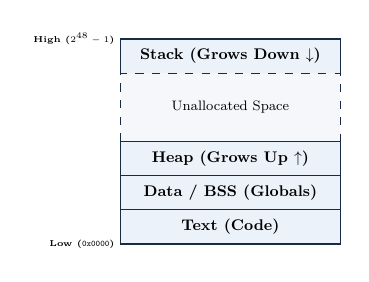
\begin{tikzpicture}[scale=0.62, every node/.style={transform shape}]
  \draw[fill=lightblue, draw=navy] (0,4.0) rectangle (4.5,4.7) node[midway, font=\small\bfseries] {Stack (Grows Down $\downarrow$)};
  \draw[fill=softgray, draw=navy, dashed] (0,2.6) rectangle (4.5,4.0) node[midway, font=\footnotesize] {Unallocated Space};
  \draw[fill=lightblue, draw=navy] (0,1.9) rectangle (4.5,2.6) node[midway, font=\small\bfseries] {Heap (Grows Up $\uparrow$)};
  \draw[fill=lightblue, draw=navy] (0,1.2) rectangle (4.5,1.9) node[midway, font=\small\bfseries] {Data / BSS (Globals)};
  \draw[fill=lightblue, draw=navy] (0,0.5) rectangle (4.5,1.2) node[midway, font=\small\bfseries] {Text (Code)};
  \node[anchor=east, font=\tiny\bfseries] at (0,4.7) {High ($2^{48}-1$)};
  \node[anchor=east, font=\tiny\bfseries] at (0,0.5) {Low (\hex{0000})};
\end{tikzpicture}
\end{column}
\end{columns}

\vfill
\begin{block}{Stack-Heap Isolation}
\small The unallocated address space ensures the stack and heap grow independently. Unchecked recursion causes the stack to exhaust this boundary, generating a segmentation fault.
\end{block}
\vfill
\end{frame}

% ============================================================
% Section 4 Divider
% ============================================================

\sectiondivider{PART 4}{Foundational Instruction Classes}

% ============================================================
% Slide 18
% ============================================================

\begin{frame}{Instruction Syntax Conventions}
\vfill
\begin{itemize}\setlength{\itemsep}{4pt}
  \item Standard AArch64 assembly strictly follows: \code{mnemonic  dst, src1, src2\_or\_imm}
  \item \key{Three-Operand Format:} Computation preserves source registers without overwriting them.
\end{itemize}

\vfill
\begin{center}
\small
\renewcommand{\arraystretch}{0.98}
\begin{tabular}{lll}
\toprule
\textbf{Assembly Example} & \textbf{RTL Operation} & \textbf{Description} \\
\midrule
\code{add x0, x1, x2}     & $x_0 \leftarrow x_1 + x_2$             & 64-bit register addition \\
\code{add w0, w1, w2}     & $w_0 \leftarrow w_1 + w_2$             & 32-bit addition (clears upper 32 bits of $x_0$) \\
\code{add x0, x1, \#16}   & $x_0 \leftarrow x_1 + 16$              & Addition with immediate constant \\
\bottomrule
\end{tabular}
\end{center}

\vfill
\begin{block}{Non-Destructive Architecture}
\small Unlike x86's destructive two-operand syntax (\code{add eax, ebx} modifies \code{eax}), AArch64 retains original operand values post-computation by routing results to an explicit destination register.
\end{block}
\vfill
\end{frame}

% ============================================================
% Slide 19
% ============================================================

\begin{frame}{Arithmetic Instructions: Addition \& Subtraction}
\vfill
\begin{center}
\small
\renewcommand{\arraystretch}{0.95}
\setlength{\tabcolsep}{5pt}
\begin{tabular}{lll}
\toprule
\textbf{Instruction} & \textbf{Operation} & \textbf{Flags Updated?} \\
\midrule
\code{add  xd, xn, xm}  & $x_d \leftarrow x_n + x_m$ & No \\
\code{adds xd, xn, xm}  & $x_d \leftarrow x_n + x_m$ & \key{Yes (Updates NZCV)} \\
\code{sub  xd, xn, xm}  & $x_d \leftarrow x_n - x_m$ & No \\
\code{subs xd, xn, xm}  & $x_d \leftarrow x_n - x_m$ & \key{Yes (Updates NZCV)} \\
\code{neg  xd, xm}      & $x_d \leftarrow 0 - x_m$ (Alias: \code{sub xd, xzr, xm}) & No \\
\code{negs xd, xm}      & $x_d \leftarrow 0 - x_m$ (Alias: \code{subs xd, xzr, xm}) & \key{Yes} \\
\bottomrule
\end{tabular}
\end{center}

\vfill
\begin{block}{Immediate Scaling}
\small Immediate values (\code{\#imm12}) span $0\text{ to }4095$ and can be natively shifted left by 12 bits in hardware via \code{lsl \#12} without extra instruction cycles.
\end{block}
\vfill
\end{frame}

% ============================================================
% Slide 20
% ============================================================

\begin{frame}{Logical Operations: Bitwise Manipulation}
\vfill
\begin{itemize}\setlength{\itemsep}{3pt}
  \item Bitwise operations execute concurrently across all 64 parallel bit slices in the ALU.
\end{itemize}

\vfill
\begin{center}
\small
\renewcommand{\arraystretch}{0.95}
\setlength{\tabcolsep}{6pt}
\begin{tabular}{lll}
\toprule
\textbf{Mnemonic} & \textbf{Operation} & \textbf{Bitwise Logic} \\
\midrule
\code{and  xd, xn, xm}  & Bitwise AND & $x_d \leftarrow x_n \land x_m$ \\
\code{orr  xd, xn, xm}  & Bitwise OR  & $x_d \leftarrow x_n \lor x_m$ \\
\code{eor  xd, xn, xm}  & Bitwise XOR & $x_d \leftarrow x_n \oplus x_m$ \\
\code{bic  xd, xn, xm}  & Bit Clear (AND NOT) & $x_d \leftarrow x_n \land (\sim x_m)$ \\
\code{mvn  xd, xm}      & Bitwise NOT & $x_d \leftarrow \sim x_m$ \\
\code{ands xd, xn, xm}  & Bitwise AND with Flags & $x_d \leftarrow x_n \land x_m \to \text{NZCV}$ \\
\bottomrule
\end{tabular}
\end{center}

\vfill
\begin{block}{Bit Clear (\texttt{bic}) Utility}
\small \code{bic x0, x1, x2} acts as a hardware mask, clearing every bit in $x_1$ where the corresponding bit in $x_2$ is \bits{1}.
\end{block}
\vfill
\end{frame}

% ============================================================
% Slide 21
% ============================================================

\begin{frame}{Shift Operations: Barrel Shifter Integration}
\vfill
\begin{itemize}\setlength{\itemsep}{3pt}
  \item AArch64 hardware integrates a dedicated \key{barrel shifter} onto the second operand datapath.
  \item Shift instructions execute standalone or fold directly into primary ALU operations.
\end{itemize}

\vfill
\begin{center}
\small
\renewcommand{\arraystretch}{1.0}
\setlength{\tabcolsep}{6pt}
\begin{tabular}{lll}
\toprule
\textbf{Mnemonic} & \textbf{Operation Name} & \textbf{Mathematical Meaning} \\
\midrule
\code{lsl xd, xn, \#k} & Logical Shift Left  & $x_d \leftarrow x_n \ll k$ (Multiplication by $2^k$) \\
\code{lsr xd, xn, \#k} & Logical Shift Right & $x_d \leftarrow x_n \gg k$ (Unsigned division by $2^k$, zero-fill) \\
\code{asr xd, xn, \#k} & Arithmetic Shift Right & $x_d \leftarrow x_n \gg k$ (Signed division by $2^k$, sign-fill) \\
\code{ror xd, xn, \#k} & Rotate Right        & Circular right bit rotation \\
\bottomrule
\end{tabular}
\end{center}

\vfill
\begin{block}{Integrated Shifted Register Example}
\small \code{add x0, x1, x2, lsl \#3} $\implies x_0 \leftarrow x_1 + (x_2 \times 8)$ executes as a \key{single instruction with hardware shift} at zero clock penalty.
\end{block}
\vfill
\end{frame}

% ============================================================
% Slide 22
% ============================================================

\begin{frame}{Comparison and Testing Instructions}
\vfill
\begin{itemize}\setlength{\itemsep}{3pt}
  \item Comparison instructions evaluate operands, update NZCV flags, and discard the numerical result.
\end{itemize}

\vfill
\begin{center}
\footnotesize
\renewcommand{\arraystretch}{1.0}
\setlength{\tabcolsep}{6pt}
\begin{tabular}{lll}
\toprule
\textbf{Instruction} & \textbf{Underlying Operation} & \textbf{Flags Updated} \\
\midrule
\code{cmp  xn, xm}      & \code{subs xzr, xn, xm}   & Evaluates $x_n - x_m \to \text{NZCV}$ \\
\code{cmn  xn, xm}      & \code{adds xzr, xn, xm}   & Evaluates $x_n + x_m \to \text{NZCV}$ (Compare Negative) \\
\code{tst  xn, xm}      & \code{ands xzr, xn, xm}   & Evaluates $x_n \land x_m \to \text{NZCV}$ (Bit Test) \\
\bottomrule
\end{tabular}
\end{center}

\vfill
\begin{block}{Flag Interpretation Rules}
\small If $x_n == x_m$, \code{cmp} asserts \key{Z (Zero)} since $x_n - x_m = 0$. If $x_n < x_m$ (signed), \code{cmp} configures flags such that $\text{N} \neq \text{V}$ (Negative differs from Overflow).
\end{block}
\vfill
\end{frame}

% ============================================================
% Slide 23
% ============================================================

\begin{frame}{Loading Immediate Constants: \texttt{movz}, \texttt{movk}, \texttt{movn}}
\vfill
\begin{itemize}\setlength{\itemsep}{3pt}
  \item A fixed 32-bit instruction cannot fit an arbitrary 64-bit constant.
  \item AArch64 constructs large constants in 16-bit chunks using \key{wide-immediate instructions}:
\end{itemize}

\vfill
\begin{center}
\footnotesize
\renewcommand{\arraystretch}{0.95}
\setlength{\tabcolsep}{4pt}
\begin{tabular}{lll}
\toprule
\textbf{Instruction} & \textbf{Operation Name} & \textbf{Semantic Action} \\
\midrule
\code{movz xd, imm, lsl s} & Move Wide with Zero & Loads 16-bit constant at shift $s$; clears other bits \\
\code{movk xd, imm, lsl s} & Move Wide with Keep & Overwrites 16 bits at shift $s$; \key{keeps} other bits intact \\
\code{movn xd, imm, lsl s} & Move Wide with NOT  & Loads bitwise inverted 16-bit constant directly \\
\bottomrule
\end{tabular}
\end{center}

\vfill
\begin{block}{Constructing a 32-bit Value (\hex{1234abcd})}
\footnotesize
\begin{tabular}{lll}
\code{movz x0, \#0xabcd}           & $\implies x_0 = \hex{000000000000abcd}$ & (Lower 16 bits loaded) \\
\code{movk x0, \#0x1234, lsl \#16} & $\implies x_0 = \hex{000000001234abcd}$ & (Bits 31:16 overwritten) \\
\end{tabular}
\end{block}
\vfill
\end{frame}

% ============================================================
% Slide 24
% ============================================================

\begin{frame}{Memory Access: Basic Load/Store Architecture}
\vfill
\begin{itemize}\setlength{\itemsep}{3pt}
  \item Memory is accessed universally via explicit load (\code{ldr}) and store (\code{str}) mechanisms.
  \item The register size specifier strictly dictates the physical data transfer width:
\end{itemize}

\vfill
\begin{center}
\footnotesize
\renewcommand{\arraystretch}{0.95}
\setlength{\tabcolsep}{4pt}
\begin{tabular}{llll}
\toprule
\textbf{Instruction} & \textbf{Register} & \textbf{Transfer Width} & \textbf{Action} \\
\midrule
\code{ldr  xt, [xn]} & 64-bit (\bits{xt}) & 8 Bytes (Doubleword) & $x_t \leftarrow \text{Mem}_8[x_n]$ \\
\code{str  xt, [xn]} & 64-bit (\bits{xt}) & 8 Bytes (Doubleword) & $\text{Mem}_8[x_n] \leftarrow x_t$ \\
\code{ldr  wt, [xn]} & 32-bit (\bits{wt}) & 4 Bytes (Word)       & $w_t \leftarrow \text{Mem}_4[x_n]$ (Zero-extended) \\
\code{str  wt, [xn]} & 32-bit (\bits{wt}) & 4 Bytes (Word)       & $\text{Mem}_4[x_n] \leftarrow w_t$ \\
\code{ldrb wt, [xn]} & 8-bit  (\bits{wt}) & 1 Byte               & $w_t \leftarrow \text{Mem}_1[x_n]$ (Zero-extended) \\
\code{strb wt, [xn]} & 8-bit  (\bits{wt}) & 1 Byte               & $\text{Mem}_1[x_n] \leftarrow w_t[7:0]$ \\
\bottomrule
\end{tabular}
\end{center}

\vfill
\begin{block}{Pointer Referencing}
\small The base register ($x_n$) holds the 64-bit memory pointer, explicitly enclosed in brackets \code{[xn]} to denote architectural indirection.
\end{block}
\vfill
\end{frame}

% ============================================================
% Slide 25
% ============================================================

\begin{frame}{Addressing Modes: Base with Immediate Offset}
\vfill
\begin{columns}[T]
\begin{column}{0.48\textwidth}
\begin{block}{Mechanism ($\text{EA} = x_n + \text{offset}$)}
\small
\begin{itemize}\setlength{\itemsep}{3pt}
  \item Syntax: \code{ldr xt, [xn, \#offset]}
  \item Accesses memory at $x_n + \text{offset}$.
  \item \key{No side effects:} Base register $x_n$ remains unchanged post-execution.
\end{itemize}
\end{block}
\end{column}

\begin{column}{0.48\textwidth}
\begin{block}{Code Examples}
\small
\begin{tabular}{ll}
\code{ldr x1, [x0]}      & \text{\scriptsize Load $[x_0]$} \\
\code{ldr x2, [x0, \#8]}  & \text{\scriptsize Load $[x_0 + 8]$} \\
\code{str x2, [x0, \#16]} & \text{\scriptsize Store $[x_0 + 16]$} \\
\end{tabular}
\end{block}
\end{column}
\end{columns}

\vfill
\begin{block}{Hardware Offset Range}
\small Unsigned 12-bit offsets scale by operand size. For 64-bit doublewords, the hardware scales by 8, yielding a maximum effective offset of $+32760$ bytes.
\end{block}
\vfill
\end{frame}

% ============================================================
% Slide 26
% ============================================================

\begin{frame}{Advanced Addressing: Pre- and Post-Indexed}
\vfill
\begin{columns}[T]
\begin{column}{0.48\textwidth}
\begin{block}{Pre-Indexed (\texttt{!})}
\small
$$\code{ldr xt, [xn, \#imm]!}$$
\begin{enumerate}\setlength{\itemsep}{2pt}
  \item Update base: $x_n \leftarrow x_n + \text{imm}$.
  \item Load memory: $x_t \leftarrow \text{Mem}[x_n]$.
\end{enumerate}
Base update happens \emph{before} access.
\end{block}
\end{column}

\begin{column}{0.48\textwidth}
\begin{block}{Post-Indexed}
\small
$$\code{ldr xt, [xn], \#imm}$$
\begin{enumerate}\setlength{\itemsep}{2pt}
  \item Load memory: $x_t \leftarrow \text{Mem}[x_n]$.
  \item Update base: $x_n \leftarrow x_n + \text{imm}$.
\end{enumerate}
Base update happens \emph{after} access.
\end{block}
\end{column}
\end{columns}

\vfill
\begin{block}{Efficiency Impact}
\small Pointer tracking integrates directly into memory instructions, eliminating separate \code{add} overhead when traversing arrays or managing stack frames.
\end{block}
\vfill
\end{frame}

% ============================================================
% Slide 27
% ============================================================

\begin{frame}[fragile]{Loading and Storing Pairs (\texttt{ldp} and \texttt{stp})}
\vfill
\begin{itemize}\setlength{\itemsep}{4pt}
  \item \key{Core Purpose:} Transfer two adjacent 64-bit registers in a single instruction.
  \item \key{Primary Use Case (Stack Management):}
  \begin{itemize}\setlength{\itemsep}{2pt}
    \item Combines two register movements into one atomic 128-bit memory operation.
    \item Saves/restores Frame Pointer ($x_{29}$) and Link Register ($x_{30}$) efficiently during calls.
  \end{itemize}
  \item \key{Performance Impact:} Issues a unified 128-bit bus transaction, doubling throughput.
\end{itemize}

\vfill
\begin{block}{Stack Frame Construction Example}
\small
\begin{verbatim}
// Push FP (x29) and LR (x30) to stack, pre-decrementing SP by 16 bytes
stp x29, x30, [sp, #-16]! 
\end{verbatim}
\end{block}
\vfill
\end{frame}

% ============================================================
% Slide 28
% ============================================================

\begin{frame}{Control Flow: Unconditional Branches}
\vfill
\begin{itemize}\setlength{\itemsep}{3pt}
  \item Control flow instructions redirect program execution by modifying the Program Counter (\bits{pc}).
\end{itemize}

\vfill
\begin{center}
\footnotesize
\renewcommand{\arraystretch}{1.02}
\setlength{\tabcolsep}{5pt}
\begin{tabular}{lll}
\toprule
\textbf{Instruction} & \textbf{Name / Syntax} & \textbf{Operational Behavior} \\
\midrule
\code{b   label}     & Direct Branch        & $\text{pc} \leftarrow \text{label}$ (PC-relative range: $\pm 128\text{ MB}$) \\
\code{br  xn}        & Indirect Branch      & $\text{pc} \leftarrow x_n$ (Jump to address held in register $x_n$) \\
\code{bl  label}     & Branch with Link     & $x_{30} \leftarrow \text{pc} + 4$; $\text{pc} \leftarrow \text{label}$ (Subroutine call) \\
\code{blr xn}        & Indirect Call        & $x_{30} \leftarrow \text{pc} + 4$; $\text{pc} \leftarrow x_n$ (Function pointer call) \\
\code{ret}           & Subroutine Return    & $\text{pc} \leftarrow x_{30}$ (Default return via Link Register) \\
\bottomrule
\end{tabular}
\end{center}

\vfill
\begin{block}{PC-Relative Addressing}
\small Direct branch offsets encode as signed displacements relative to current \bits{pc}, guaranteeing compiled machine code executes regardless of where it is mapped in memory.
\end{block}
\vfill
\end{frame}

% ============================================================
% Slide 29
% ============================================================

\begin{frame}{Conditional Branches \& Condition Codes}
\vfill
\small Syntax: \code{b.cond label} (Branches to \code{label} only if the condition evaluates to true).

\vfill
\begin{center}
\footnotesize
\renewcommand{\arraystretch}{0.92}
\setlength{\tabcolsep}{5pt}
\begin{tabular}{llll}
\toprule
\textbf{Condition Code} & \textbf{Meaning} & \textbf{Flag Condition} & \textbf{Comparison Context} \\
\midrule
\code{b.eq} & Equal / Zero               & $\text{Z} == 1$ & Signed / Unsigned \\
\code{b.ne} & Not Equal / Non-Zero       & $\text{Z} == 0$ & Signed / Unsigned \\
\code{b.lt} & Signed Less Than           & $\text{N} \neq \text{V}$ & Signed \\
\code{b.le} & Signed Less Than or Equal  & $(\text{Z} == 1) \lor (\text{N} \neq \text{V})$ & Signed \\
\code{b.gt} & Signed Greater Than        & $(\text{Z} == 0) \land (\text{N} == \text{V})$ & Signed \\
\code{b.ge} & Signed Greater or Equal    & $\text{N} == \text{V}$ & Signed \\
\code{b.lo} & Unsigned Lower ($<$)       & $\text{C} == 0$ & Unsigned \\
\code{b.hi} & Unsigned Higher ($>$)      & $(\text{C} == 1) \land (\text{Z} == 0)$ & Unsigned \\
\bottomrule
\end{tabular}
\end{center}

\vfill
\begin{block}{Branch Prediction Context}
\small Unpredictable conditional branches stall superscalar pipelines. Processors mitigate this penalty using hardware branch predictors and branch target buffers (BTB).
\end{block}
\vfill
\end{frame}

% ============================================================
% Slide 30
% ============================================================

\begin{frame}[fragile]{Control Flow Idiom: If-Else Translation}
\vfill
\begin{columns}[T]
\begin{column}{0.44\textwidth}
\begin{block}{High-Level C Code}
\small
\begin{verbatim}
if (a == b) {
    c = c + 1;
} else {
    c = c - 1;
}
\end{verbatim}
\end{block}
\end{column}

\begin{column}{0.52\textwidth}
\begin{block}{AArch64 Assembly Mapping}
\small
\begin{tabular}{ll}
\multicolumn{2}{l}{\textit{// Assume: x0=a, x1=b, x2=c}} \\
\code{cmp  x0, x1}        & \text{\scriptsize // Compare a and b} \\
\code{b.ne .Lelse}        & \text{\scriptsize // If a != b, jump to else} \\
\code{add  x2, x2, \#1}   & \text{\scriptsize // Then-body: c = c + 1} \\
\code{b    .Lend}         & \text{\scriptsize // Skip else-body} \\
\code{.Lelse:}            & \\
\code{sub  x2, x2, \#1}   & \text{\scriptsize // Else-body: c = c - 1} \\
\code{.Lend:}             & \\
\end{tabular}
\end{block}
\end{column}
\end{columns}

\vfill
\begin{block}{Assembly Inversion Pattern}
\small High-level conditions invert their test in compiled assembly to branch \emph{around} the positive then-body directly to the alternative path.
\end{block}
\vfill
\end{frame}

% ============================================================
% Slide 31
% ============================================================

\begin{frame}[fragile]{Control Flow Idiom: While-Loop Translation}
\vfill
\begin{columns}[T]
\begin{column}{0.44\textwidth}
\begin{block}{High-Level C Loop}
\scriptsize
\begin{verbatim}
// Compute sum of array
uint64_t i = 0;
while (i < n) {
    sum += arr[i];
    i++;
}
\end{verbatim}
\end{block}
\end{column}

\begin{column}{0.54\textwidth}
\begin{block}{AArch64 Assembly Translation}
\scriptsize
\setlength{\tabcolsep}{2pt}
\begin{tabular}{ll}
\multicolumn{2}{l}{\textit{// x0=arr, x1=n, x2=i, x3=sum}} \\
\code{mov  x2, xzr}       & \text{\tiny // i = 0} \\
\code{mov  x3, xzr}       & \text{\tiny // sum = 0} \\
\code{.Lloop:}            & \\
\code{cmp  x2, x1}        & \text{\tiny // Test i < n} \\
\code{b.ge .Ldone}        & \text{\tiny // Exit if i >= n} \\
\code{ldr  x4, [x0, x2, lsl \#3]} & \text{\tiny // Load arr[i]} \\
\code{add  x3, x3, x4}    & \text{\tiny // sum += arr[i]} \\
\code{add  x2, x2, \#1}   & \text{\tiny // i++} \\
\code{b    .Lloop}        & \text{\tiny // Repeat loop} \\
\code{.Ldone:}            & \\
\end{tabular}
\end{block}
\end{column}
\end{columns}

\vfill
\begin{block}{Optimization Note}
\small Compilers unroll loop bodies to eliminate jumping instructions and amortize branch penalties over multiple iterations.
\end{block}
\vfill
\end{frame}

% ============================================================
% Slide 32
% ============================================================

\begin{frame}{Conditional Select Instructions: Eliminating Branches}
\vfill
\begin{itemize}\setlength{\itemsep}{3pt}
  \item Branch instructions introduce branch misprediction penalties.
  \item AArch64 deploys \key{conditional select instructions} to choose operands branchlessly:
\end{itemize}

\vfill
\begin{center}
\small
\renewcommand{\arraystretch}{0.98}
\setlength{\tabcolsep}{6pt}
\begin{tabular}{lll}
\toprule
\textbf{Instruction} & \textbf{Semantic Operation} & \textbf{C Ternary Equivalent} \\
\midrule
\code{csel  xd, xn, xm, cond} & $x_d \leftarrow \text{cond} \mathbin{?} x_n : x_m$ & \code{d = cond ? n : m;} \\
\code{cinc  xd, xn, cond}       & $x_d \leftarrow \text{cond} \mathbin{?} (x_n + 1) : x_n$ & \code{d = n + (cond ? 1 : 0);} \\
\code{cset  xd, cond}           & $x_d \leftarrow \text{cond} \mathbin{?} 1 : 0$ & \code{d = (cond) ? 1 : 0;} \\
\bottomrule
\end{tabular}
\end{center}

\vfill
\begin{block}{Branchless Maximum: $\max(x_1, x_2)$}
\small
\begin{tabular}{ll}
\code{cmp  x1, x2}         & \text{\scriptsize // Compare x1 and x2} \\
\code{csel x0, x1, x2, gt} & \text{\scriptsize // If x1 > x2, x0 = x1; else x0 = x2 (0 branch penalties)} \\
\end{tabular}
\end{block}
\vfill
\end{frame}

% ============================================================
% Section 5 Divider
% ============================================================

\sectiondivider{SUMMARY \& ASSESSMENT}{Review and Self-Test Questions}

% ============================================================
% Slide 33: Comprehensive Summary
% ============================================================

\begin{frame}{Topic 3: Comprehensive Summary}
\vfill
\begin{itemize}\setlength{\itemsep}{7pt}
  \item \key{Architectural State:} Precise hardware-software contract defined by general registers (\bits{x0}--\bits{x30}), flags (NZCV), stack pointer (\bits{sp}), program counter (\bits{pc}), and byte-addressed memory.
  \item \key{Register Structure:} 31 orthogonal 64-bit registers (\bits{x0}--\bits{x30}) alias 32-bit views (\bits{w0}--\bits{w30}); writing to a \bits{w} register automatically clears the upper 32 bits.
  \item \key{ABI Rules:} \bits{x0}--\bits{x7} handle arguments/returns (caller-saved); \bits{x19}--\bits{x28} hold local variables across calls (callee-saved).
  \item \key{Load/Store Operations:} Arithmetic occurs exclusively in registers; memory access is restricted to \code{ldr}/\code{str} offset, indexed, or paired (\code{ldp}/\code{stp}) instructions.
  \item \key{Control Flow:} Branching evaluates NZCV flags updated by \code{adds}/\code{subs}/\code{cmp}; conditional select (\code{csel}) eliminates branch penalties entirely.
\end{itemize}
\vfill
\end{frame}

% ============================================================
% Slide 34: Self-Test Questions (Part 1)
% ============================================================

\begin{frame}{Self-Test Questions: State \& Register Mechanics}
\vfill
\begin{enumerate}\setlength{\itemsep}{8pt}
  \item \key{Architectural vs.\ Microarchitectural State:} Why are CPU branch prediction tables and physical register rename structures classified as microarchitectural state rather than architectural state?

  \item \key{32-bit Register Write Semantics:} Suppose register \bits{x5} initially contains \hex{ffffffff\_ffffffff}. If the instruction \code{mov w5, \#0x1234} is executed, what exact 64-bit value resides in \bits{x5} post-execution?

  \item \key{Zero Register Application:} Why does AArch64 provide a dedicated zero register (\bits{xzr}/\bits{wzr}) instead of permanently assigning a general-purpose register (like \bits{x0}) to hold zero?

  \item \key{Calling Convention Responsibility:} If function \code{foo()} calls \code{bar()}, and \code{foo()} needs to preserve values across the call in registers \bits{x3} and \bits{x20}, which function is responsible for saving each register to the stack?
\end{enumerate}
\vfill
\end{frame}

% ============================================================
% Slide 35: Self-Test Questions (Part 2)
% ============================================================

\begin{frame}{Self-Test Questions: Memory \& Instruction Mechanics}
\vfill
\begin{enumerate}\setlength{\itemsep}{7pt}
  \item \key{Memory Addressing Modes:} Explain the mechanical difference in address calculation and base register updates between: \code{ldr x1, [x0, \#16]} vs.\ \code{ldr x1, [x0, \#16]!} vs.\ \code{ldr x1, [x0], \#16}.

  \item \key{Endianness Evaluation:} The 32-bit word \hex{deadbeef} is stored at address \hex{2000} on a little-endian AArch64 machine. What exact byte is stored at address \hex{2000}? At address \hex{2003}?

  \item \key{Branch Elimination via \texttt{csel}:} Convert this C statement into branchless assembly using \code{cmp} and \code{csel}:\\
  \code{int64\_t result = (val1 <= val2) ? (val1 + 10) : (val2 - 5);}

  \item \key{Condition Flag Verification:} If \bits{x0} contains $5$ and \bits{x1} contains $10$, which NZCV flags are asserted ($=1$) following \code{cmp x0, x1}?
\end{enumerate}
\vfill
\end{frame}

% ============================================================
% Slide 36: Look Ahead
% ============================================================

\begin{frame}{Looking Ahead to Topic 4: Assembly Programming}
\vfill
\begin{block}{Topic 4 Preview (Arithmetic, Logic, \& Control Flow)}
Moving from architectural structure to assembly implementation.
\end{block}

\vfill
\begin{itemize}\setlength{\itemsep}{6pt}
  \item \key{ALU \& Barrel Shifting:} Complex arithmetic paired with zero-penalty second-operand hardware shifts.
  \item \key{Bitwise Logic \& Field Extraction:} Manipulating bitfields using masks, bit clears (\code{bic}), and bitfield extracts (\code{ubfx}).
  \item \key{Condition Flags \& Comparisons:} Leveraging NZCV flags and choosing between signed vs.\ unsigned branch conditions.
  \item \key{Control Flow \& Branchless Selection:} Translating loops and nested conditionals while using \code{csel} to bypass branch prediction penalties.
\end{itemize}
\vfill
\end{frame}

\end{document}